\documentclass[12pt]{article}
\usepackage[margin=.5 in]{geometry}
\usepackage{fontspec}
\usepackage[english]{babel} 
\newfontfamily\skt[Script=Devanagari]{Adobe Devanagari}
\newfontfamily\sktr[Script=Devanagari]{Adishila}
\usepackage{parskip}
\usepackage{graphicx}
\graphicspath{ {images/} }
\usepackage{float}
\usepackage{wrapfig}
\usepackage{array}
\usepackage{amsmath}
\usepackage{amssymb}
\usepackage{array}
\usepackage{parskip}
\usepackage[table, dvipsnames]{xcolor}
\usepackage{tikz}
\usepackage{tikz-network}
\usetikzlibrary{arrows, arrows.meta, patterns, shapes.geometric, shapes.misc, graphs, mindmap, calc}
\title{\textbf{Exoplanet orbits}}
\author{}
\date{}

\begin{document}
	\maketitle
\begin{center}
\begin{tikzpicture} 
\draw (0,0) ellipse [x radius=0.387, y radius=0.3787322]; %Mercury
\draw (0,0) ellipse [x radius=0.723, y radius=0.7229838];  %Venus
\draw (0,0) ellipse [x radius=1, y radius=0.9998605]; %Earth
\draw (0,0) ellipse [x radius=1.524, y radius=1.517324]; %Mars
\draw (0,0) ellipse [x radius=5.204, y radius=5.197774]; %Jupiter
\draw (0,0) ellipse [x radius=9.583, y radius=9.567692]; %Saturn
\draw[Goldenrod, fill=Goldenrod] (-0.01671022,0) circle [radius=0.1]; \node[Gray] at (0,-9.567692)[below] {Saturn=10759.22 days};\node[CadetBlue] at (0,9.567692)[above] {Solar System: Mercury..Saturn};\end{tikzpicture}
\newpage
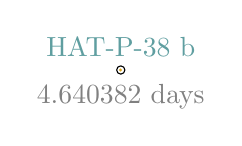
\begin{tikzpicture} \draw (0,0) ellipse [x radius=0.05231, y radius=0.05223082]; \draw[Goldenrod, fill=Goldenrod] (-0.00287705,0) circle [radius=0.01]; \node[Gray] at (0,-0.05223082)[below] {4.640382 days};\node[CadetBlue] at (0,0.05223082)[above] {HAT-P-38 b};\end{tikzpicture}
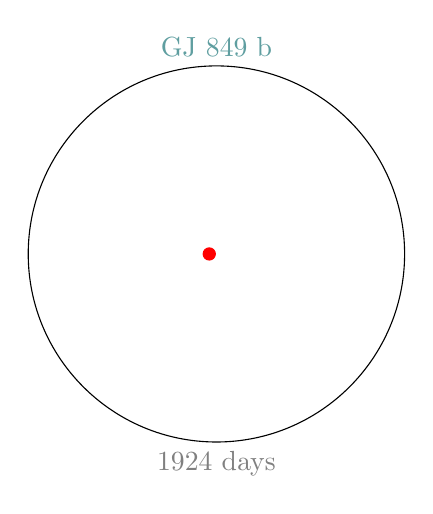
\begin{tikzpicture} \draw (0,0) ellipse [x radius=2.39, y radius=2.388274]; \draw[Red, fill=Red] (-0.09082,0) circle [radius=0.07719443]; \node[Gray] at (0,-2.388274)[below] {1924 days};\node[CadetBlue] at (0,2.388274)[above] {GJ 849 b};\end{tikzpicture}
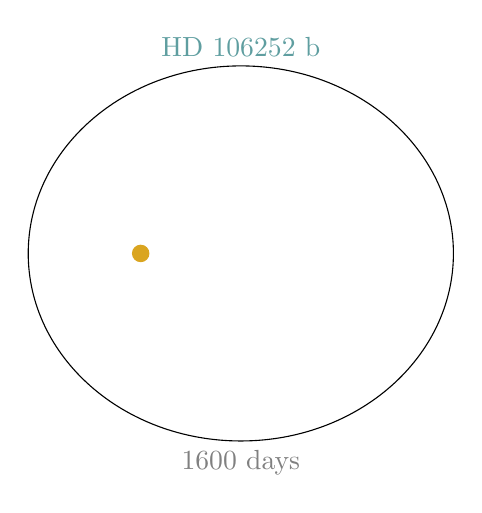
\begin{tikzpicture} \draw (0,0) ellipse [x radius=2.7, y radius=2.38176]; \draw[Goldenrod, fill=Goldenrod] (-1.2717,0) circle [radius=0.1038499]; \node[Gray] at (0,-2.38176)[below] {1600 days};\node[CadetBlue] at (0,2.38176)[above] {HD 106252 b};\end{tikzpicture}
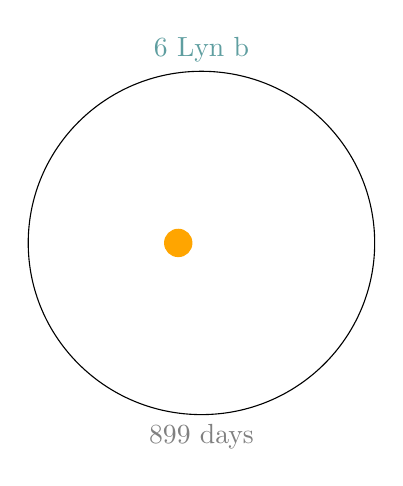
\begin{tikzpicture} \draw (0,0) ellipse [x radius=2.2, y radius=2.180159]; \draw[Orange, fill=Orange] (-0.2948,0) circle [radius=0.1732478]; \node[Gray] at (0,-2.180159)[below] {899 days};\node[CadetBlue] at (0,2.180159)[above] {6 Lyn b};\end{tikzpicture}
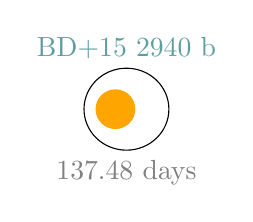
\begin{tikzpicture} \draw (0,0) ellipse [x radius=0.539, y radius=0.520463]; \draw[Orange, fill=Orange] (-0.14014,0) circle [radius=0.244966]; \node[Gray] at (0,-0.520463)[below] {137.48 days};\node[CadetBlue] at (0,0.520463)[above] {BD+15 2940 b};\end{tikzpicture}
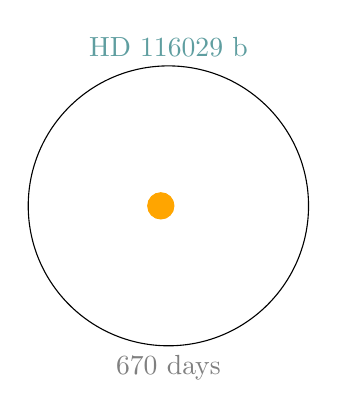
\begin{tikzpicture} \draw (0,0) ellipse [x radius=1.78, y radius=1.777403]; \draw[Orange, fill=Orange] (-0.09612,0) circle [radius=0.1663103]; \node[Gray] at (0,-1.777403)[below] {670 days};\node[CadetBlue] at (0,1.777403)[above] {HD 116029 b};\end{tikzpicture}
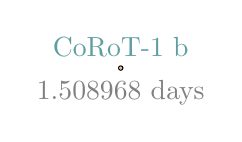
\begin{tikzpicture} \draw (0,0) ellipse [x radius=0.02752, y radius=0.02750216]; \draw[Apricot, fill=Apricot] (-0.00099072,0) circle [radius=0.01]; \node[Gray] at (0,-0.02750216)[below] {1.508968 days};\node[CadetBlue] at (0,0.02750216)[above] {CoRoT-1 b};\end{tikzpicture}
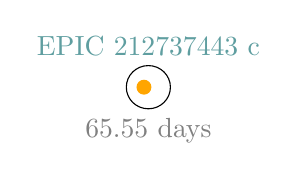
\begin{tikzpicture} \draw (0,0) ellipse [x radius=0.28, y radius=0.2743429]; \draw[Orange, fill=Orange] (-0.056,0) circle [radius=0.0875034]; \node[Gray] at (0,-0.2743429)[below] {65.55 days};\node[CadetBlue] at (0,0.2743429)[above] {EPIC 212737443 c};\end{tikzpicture}
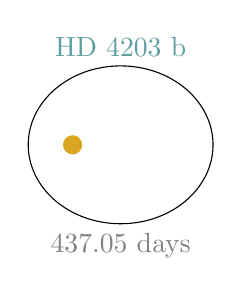
\begin{tikzpicture} \draw (0,0) ellipse [x radius=1.1735, y radius=1.002364]; \draw[Goldenrod, fill=Goldenrod] (-0.61022,0) circle [radius=0.1144714]; \node[Gray] at (0,-1.002364)[below] {437.05 days};\node[CadetBlue] at (0,1.002364)[above] {HD 4203 b};\end{tikzpicture}
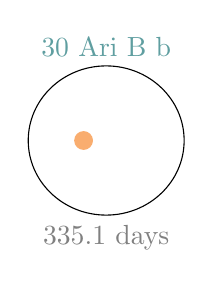
\begin{tikzpicture} \draw (0,0) ellipse [x radius=0.99, y radius=0.9474564]; \draw[Apricot, fill=Apricot] (-0.2871,0) circle [radius=0.1121346]; \node[Gray] at (0,-0.9474564)[below] {335.1 days};\node[CadetBlue] at (0,0.9474564)[above] {30 Ari B b};\end{tikzpicture}
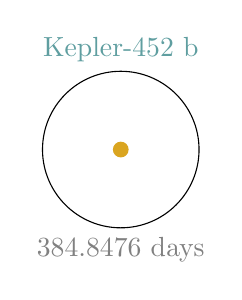
\begin{tikzpicture} \draw (0,0) ellipse [x radius=0.994, y radius=0.994]; \draw[Goldenrod, fill=Goldenrod] (0,0) circle [radius=0.09283178]; \node[Gray] at (0,-0.994)[below] {384.8476 days};\node[CadetBlue] at (0,0.994)[above] {Kepler-452 b};\end{tikzpicture}
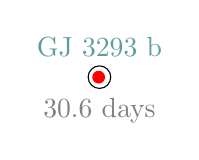
\begin{tikzpicture} \draw (0,0) ellipse [x radius=0.1434, y radius=0.1430482]; \draw[Red, fill=Red] (-0.010038,0) circle [radius=0.07368063]; \node[Gray] at (0,-0.1430482)[below] {30.6 days};\node[CadetBlue] at (0,0.1430482)[above] {GJ 3293 b};\end{tikzpicture}
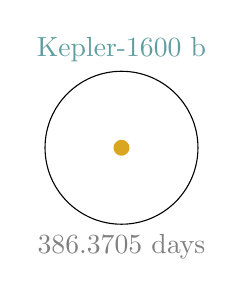
\begin{tikzpicture} \draw (0,0) ellipse [x radius=0.9712, y radius=0.9712]; \draw[Goldenrod, fill=Goldenrod] (0,0) circle [radius=0.09397796]; \node[Gray] at (0,-0.9712)[below] {386.3705 days};\node[CadetBlue] at (0,0.9712)[above] {Kepler-1600 b};\end{tikzpicture}
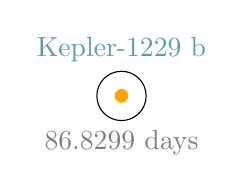
\begin{tikzpicture} \draw (0,0) ellipse [x radius=0.313, y radius=0.313]; \draw[Orange, fill=Orange] (0,0) circle [radius=0.08041452]; \node[Gray] at (0,-0.313)[below] {86.8299 days};\node[CadetBlue] at (0,0.313)[above] {Kepler-1229 b};\end{tikzpicture}
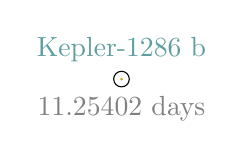
\begin{tikzpicture} \draw (0,0) ellipse [x radius=0.0991, y radius=0.0991]; \draw[Goldenrod, fill=Goldenrod] (0,0) circle [radius=0.01]; \node[Gray] at (0,-0.0991)[below] {11.25402 days};\node[CadetBlue] at (0,0.0991)[above] {Kepler-1286 b};\end{tikzpicture}
\begin{tikzpicture} \draw (0,0) ellipse [x radius=3.29347, y radius=2.913561]; \draw[Orange, fill=Orange] (-1.535613,0) circle [radius=0.09321698]; \node[Gray] at (0,-2.913561)[below] {2468.46 days};\node[CadetBlue] at (0,2.913561)[above] {HD 181433 d};\end{tikzpicture}
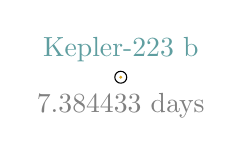
\begin{tikzpicture} \draw (0,0) ellipse [x radius=0.0756, y radius=0.0756]; \draw[Goldenrod, fill=Goldenrod] (0,0) circle [radius=0.01]; \node[Gray] at (0,-0.0756)[below] {7.384433 days};\node[CadetBlue] at (0,0.0756)[above] {Kepler-223 b};\end{tikzpicture}
\begin{tikzpicture} \draw (0,0) ellipse [x radius=3.18, y radius=3.178569]; \draw[Goldenrod, fill=Goldenrod] (-0.0954,0) circle [radius=0.1006623]; \node[Gray] at (0,-3.178569)[below] {2068 days};\node[CadetBlue] at (0,3.178569)[above] {HD 70642 b};\end{tikzpicture}
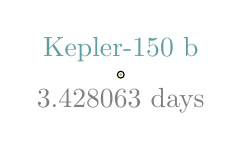
\begin{tikzpicture} \draw (0,0) ellipse [x radius=0.043, y radius=0.043]; \draw[Goldenrod, fill=Goldenrod] (0,0) circle [radius=0.01]; \node[Gray] at (0,-0.043)[below] {3.428063 days};\node[CadetBlue] at (0,0.043)[above] {Kepler-150 b};\end{tikzpicture}
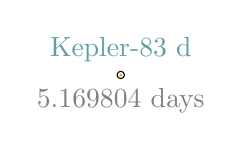
\begin{tikzpicture} \draw (0,0) ellipse [x radius=0.0467, y radius=0.0467]; \draw[Orange, fill=Orange] (0,0) circle [radius=0.01]; \node[Gray] at (0,-0.0467)[below] {5.169804 days};\node[CadetBlue] at (0,0.0467)[above] {Kepler-83 d};\end{tikzpicture}
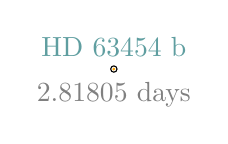
\begin{tikzpicture} \draw (0,0) ellipse [x radius=0.04, y radius=0.04]; \draw[Orange, fill=Orange] (0,0) circle [radius=0.01]; \node[Gray] at (0,-0.04)[below] {2.81805 days};\node[CadetBlue] at (0,0.04)[above] {HD 63454 b};\end{tikzpicture}
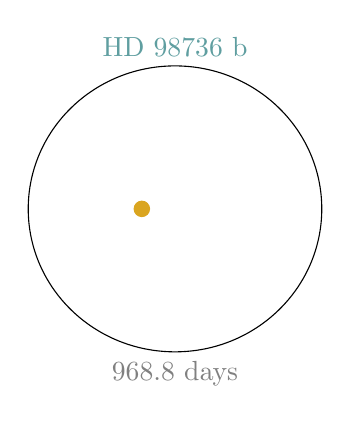
\begin{tikzpicture} \draw (0,0) ellipse [x radius=1.864, y radius=1.815773]; \draw[Goldenrod, fill=Goldenrod] (-0.421264,0) circle [radius=0.09761]; \node[Gray] at (0,-1.815773)[below] {968.8 days};\node[CadetBlue] at (0,1.815773)[above] {HD 98736 b};\end{tikzpicture}
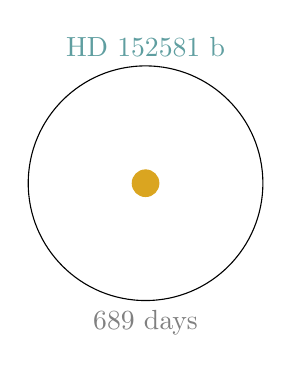
\begin{tikzpicture} \draw (0,0) ellipse [x radius=1.49, y radius=1.49]; \draw[Goldenrod, fill=Goldenrod] (0,0) circle [radius=0.1686865]; \node[Gray] at (0,-1.49)[below] {689 days};\node[CadetBlue] at (0,1.49)[above] {HD 152581 b};\end{tikzpicture}
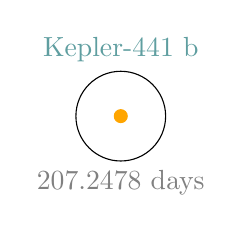
\begin{tikzpicture} \draw (0,0) ellipse [x radius=0.5697, y radius=0.5697]; \draw[Orange, fill=Orange] (0,0) circle [radius=0.08193213]; \node[Gray] at (0,-0.5697)[below] {207.2478 days};\node[CadetBlue] at (0,0.5697)[above] {Kepler-441 b};\end{tikzpicture}
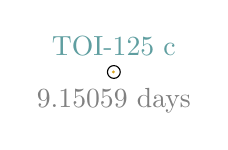
\begin{tikzpicture} \draw (0,0) ellipse [x radius=0.0814, y radius=0.08122252]; \draw[Goldenrod, fill=Goldenrod] (-0.0053724,0) circle [radius=0.01]; \node[Gray] at (0,-0.08122252)[below] {9.15059 days};\node[CadetBlue] at (0,0.08122252)[above] {TOI-125 c};\end{tikzpicture}
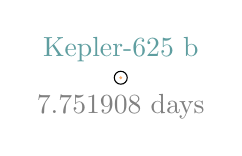
\begin{tikzpicture} \draw (0,0) ellipse [x radius=0.082, y radius=0.082]; \draw[Apricot, fill=Apricot] (0,0) circle [radius=0.01]; \node[Gray] at (0,-0.082)[below] {7.751908 days};\node[CadetBlue] at (0,0.082)[above] {Kepler-625 b};\end{tikzpicture}
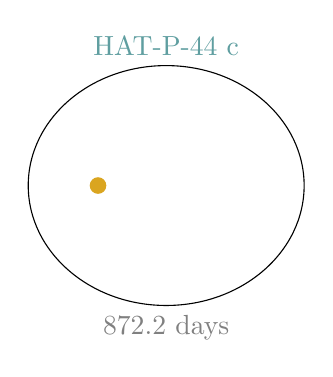
\begin{tikzpicture} \draw (0,0) ellipse [x radius=1.752, y radius=1.523297]; \draw[Goldenrod, fill=Goldenrod] (-0.865488,0) circle [radius=0.09830476]; \node[Gray] at (0,-1.523297)[below] {872.2 days};\node[CadetBlue] at (0,1.523297)[above] {HAT-P-44 c};\end{tikzpicture}
\begin{tikzpicture} \draw (0,0) ellipse [x radius=3.46, y radius=3.44891]; \draw[gray, fill=gray] (-0.2768,0) circle [radius=0.07605905]; \node[Gray] at (0,-3.44891)[below] {3507 days};\node[CadetBlue] at (0,3.44891)[above] {GJ 832 b};\end{tikzpicture}
\begin{tikzpicture} \draw (0,0) ellipse [x radius=3.242, y radius=3.209611]; \draw[Goldenrod, fill=Goldenrod] (-0.457122,0) circle [radius=0.09725888]; \node[Gray] at (0,-3.209611)[below] {2198.14 days};\node[CadetBlue] at (0,3.209611)[above] {HD 27631 b};\end{tikzpicture}
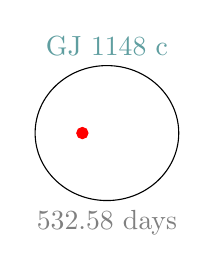
\begin{tikzpicture} \draw (0,0) ellipse [x radius=0.912, y radius=0.8570064]; \draw[Red, fill=Red] (-0.311904,0) circle [radius=0.07113787]; \node[Gray] at (0,-0.8570064)[below] {532.58 days};\node[CadetBlue] at (0,0.8570064)[above] {GJ 1148 c};\end{tikzpicture}
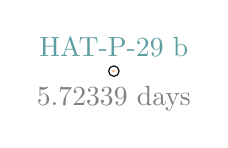
\begin{tikzpicture} \draw (0,0) ellipse [x radius=0.0665, y radius=0.0663127]; \draw[Apricot, fill=Apricot] (-0.0049875,0) circle [radius=0.01]; \node[Gray] at (0,-0.0663127)[below] {5.72339 days};\node[CadetBlue] at (0,0.0663127)[above] {HAT-P-29 b};\end{tikzpicture}
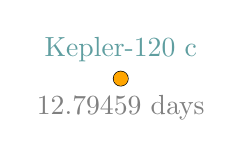
\begin{tikzpicture} \draw (0,0) ellipse [x radius=0.093, y radius=0.093]; \draw[Orange, fill=Orange] (0,0) circle [radius=0.08387207]; \node[Gray] at (0,-0.093)[below] {12.79459 days};\node[CadetBlue] at (0,0.093)[above] {Kepler-120 c};\end{tikzpicture}
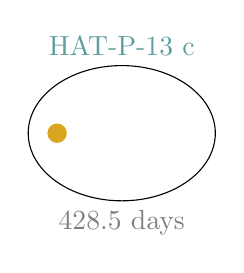
\begin{tikzpicture} \draw (0,0) ellipse [x radius=1.188, y radius=0.8587515]; \draw[Goldenrod, fill=Goldenrod] (-0.820908,0) circle [radius=0.1159778]; \node[Gray] at (0,-0.8587515)[below] {428.5 days};\node[CadetBlue] at (0,0.8587515)[above] {HAT-P-13 c};\end{tikzpicture}
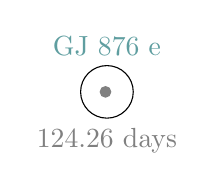
\begin{tikzpicture} \draw (0,0) ellipse [x radius=0.3343, y radius=0.333794]; \draw[gray, fill=gray] (-0.0183865,0) circle [radius=0.0669433]; \node[Gray] at (0,-0.333794)[below] {124.26 days};\node[CadetBlue] at (0,0.333794)[above] {GJ 876 e};
\end{tikzpicture}
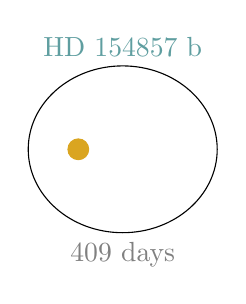
\begin{tikzpicture} \draw (0,0) ellipse [x radius=1.2, y radius=1.0592]; \draw[Goldenrod, fill=Goldenrod] (-0.564,0) circle [radius=0.1314242]; \node[Gray] at (0,-1.0592)[below] {409 days};\node[CadetBlue] at (0,1.0592)[above] {HD 154857 b};\end{tikzpicture}
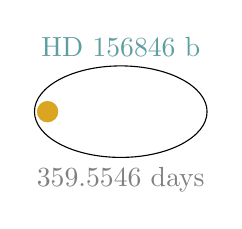
\begin{tikzpicture} \draw (0,0) ellipse [x radius=1.096, y radius=0.5811388]; \draw[Goldenrod, fill=Goldenrod] (-0.9292436,0) circle [radius=0.1284632]; \node[Gray] at (0,-0.5811388)[below] {359.5546 days};\node[CadetBlue] at (0,0.5811388)[above] {HD 156846 b};\end{tikzpicture}
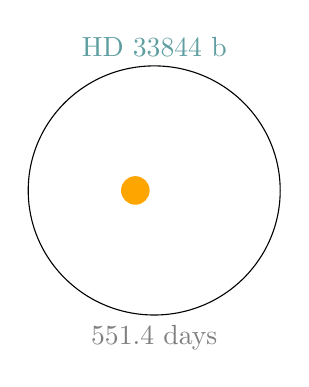
\begin{tikzpicture} \draw (0,0) ellipse [x radius=1.6, y radius=1.581898]; \draw[Orange, fill=Orange] (-0.24,0) circle [radius=0.1742416]; \node[Gray] at (0,-1.581898)[below] {551.4 days};\node[CadetBlue] at (0,1.581898)[above] {HD 33844 b};\end{tikzpicture}
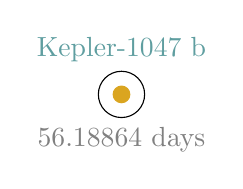
\begin{tikzpicture} \draw (0,0) ellipse [x radius=0.2939, y radius=0.2939]; \draw[Goldenrod, fill=Goldenrod] (0,0) circle [radius=0.1056722]; \node[Gray] at (0,-0.2939)[below] {56.18864 days};\node[CadetBlue] at (0,0.2939)[above] {Kepler-1047 b};\end{tikzpicture}
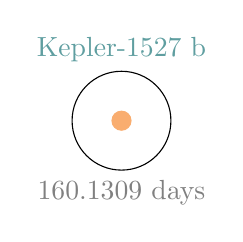
\begin{tikzpicture} \draw (0,0) ellipse [x radius=0.6276, y radius=0.6276]; \draw[Apricot, fill=Apricot] (0,0) circle [radius=0.1207362]; \node[Gray] at (0,-0.6276)[below] {160.1309 days};\node[CadetBlue] at (0,0.6276)[above] {Kepler-1527 b};\end{tikzpicture}
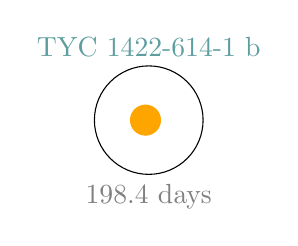
\begin{tikzpicture} \draw (0,0) ellipse [x radius=0.69, y radius=0.6887569]; \draw[Orange, fill=Orange] (-0.0414,0) circle [radius=0.1899169]; \node[Gray] at (0,-0.6887569)[below] {198.4 days};\node[CadetBlue] at (0,0.6887569)[above] {TYC 1422-614-1 b};\end{tikzpicture}
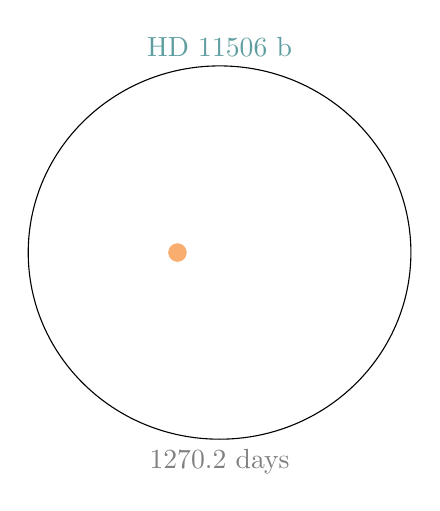
\begin{tikzpicture} \draw (0,0) ellipse [x radius=2.43, y radius=2.370465]; \draw[Apricot, fill=Apricot] (-0.5346,0) circle [radius=0.1105209]; \node[Gray] at (0,-2.370465)[below] {1270.2 days};\node[CadetBlue] at (0,2.370465)[above] {HD 11506 b};\end{tikzpicture}
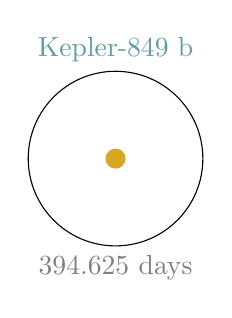
\begin{tikzpicture} \draw (0,0) ellipse [x radius=1.1088, y radius=1.1088]; \draw[Goldenrod, fill=Goldenrod] (0,0) circle [radius=0.1200463]; \node[Gray] at (0,-1.1088)[below] {394.625 days};\node[CadetBlue] at (0,1.1088)[above] {Kepler-849 b};\end{tikzpicture}
\begin{tikzpicture} \draw (0,0) ellipse [x radius=5.02, y radius=3.771353]; \draw[Apricot, fill=Apricot] (-3.3132,0) circle [radius=0.1200463]; \node[Gray] at (0,-3.771353)[below] {3638 days};\node[CadetBlue] at (0,3.771353)[above] {HD 196067 b};\end{tikzpicture}
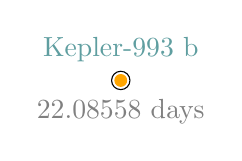
\begin{tikzpicture} \draw (0,0) ellipse [x radius=0.1165, y radius=0.1165]; \draw[Orange, fill=Orange] (0,0) circle [radius=0.07428959]; \node[Gray] at (0,-0.1165)[below] {22.08558 days};\node[CadetBlue] at (0,0.1165)[above] {Kepler-993 b};\end{tikzpicture}
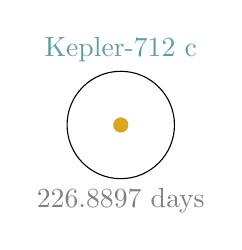
\begin{tikzpicture} \draw (0,0) ellipse [x radius=0.682, y radius=0.682]; \draw[Goldenrod, fill=Goldenrod] (0,0) circle [radius=0.08962809]; \node[Gray] at (0,-0.682)[below] {226.8897 days};\node[CadetBlue] at (0,0.682)[above] {Kepler-712 c};\end{tikzpicture}
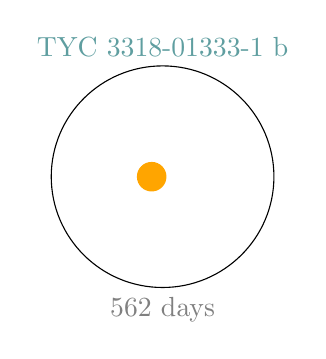
\begin{tikzpicture} \draw (0,0) ellipse [x radius=1.414, y radius=1.407194]; \draw[Orange, fill=Orange] (-0.138572,0) circle [radius=0.1806969]; \node[Gray] at (0,-1.407194)[below] {562 days};\node[CadetBlue] at (0,1.407194)[above] {TYC 3318-01333-1 b};\end{tikzpicture}
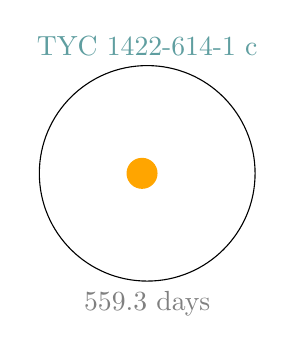
\begin{tikzpicture} \draw (0,0) ellipse [x radius=1.37, y radius=1.368421]; \draw[Orange, fill=Orange] (-0.06576,0) circle [radius=0.1899169]; \node[Gray] at (0,-1.368421)[below] {559.3 days};\node[CadetBlue] at (0,1.368421)[above] {TYC 1422-614-1 c};\end{tikzpicture}
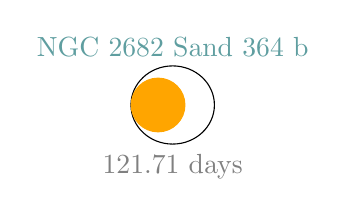
\begin{tikzpicture} \draw (0,0) ellipse [x radius=0.53, y radius=0.4964773]; \draw[Orange, fill=Orange] (-0.1855,0) circle [radius=0.3408227]; \node[Gray] at (0,-0.4964773)[below] {121.71 days};\node[CadetBlue] at (0,0.4964773)[above] {NGC 2682 Sand 364 b};\end{tikzpicture}
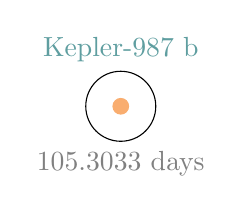
\begin{tikzpicture} \draw (0,0) ellipse [x radius=0.4445, y radius=0.4445]; \draw[Apricot, fill=Apricot] (0,0) circle [radius=0.09898983]; \node[Gray] at (0,-0.4445)[below] {105.3033 days};\node[CadetBlue] at (0,0.4445)[above] {Kepler-987 b};\end{tikzpicture}
\begin{tikzpicture} \draw (0,0) ellipse [x radius=0.4809, y radius=0.4809]; \draw[Apricot, fill=Apricot] (0,0) circle [radius=0.1035399]; \node[Gray] at (0,-0.4809)[below] {117.9311 days};\node[CadetBlue] at (0,0.4809)[above] {Kepler-807 b};\end{tikzpicture}
\begin{tikzpicture} \draw (0,0) ellipse [x radius=0.7106, y radius=0.7106]; \draw[Goldenrod, fill=Goldenrod] (0,0) circle [radius=0.09795861]; \node[Gray] at (0,-0.7106)[below] {242.4671 days};\node[CadetBlue] at (0,0.7106)[above] {Kepler-69 c};\end{tikzpicture}
\begin{tikzpicture} \draw (0,0) ellipse [x radius=0.2054, y radius=0.2054]; \draw[Goldenrod, fill=Goldenrod] (0,0) circle [radius=0.09004113]; \node[Gray] at (0,-0.2054)[below] {37.8659 days};\node[CadetBlue] at (0,0.2054)[above] {Kepler-362 c};\end{tikzpicture}
\end{center}
\end{document} 

